% !TeX root = main.tex
\clearpage
\subsection{B2: Microservicios}
\label{sec:fase6-b2}
\subsubsection{S2: Servicio de auditoría}
\label{sec:b2-auditoria}

Se implementó \texttt{audit-svc} como primer servicio del orden definido
en A5. Consume eventos durables de NATS JetStream y registra quién,
qué, cuándo y el identificador de correlación en PostgreSQL. La consulta
\path{GET /v2/audit} permite paginación y filtros por tipo de entidad,
identificador y rango de fechas con zona horaria. La implementación se
conserva en \path{cna/services/audit_svc/}; sus pruebas y despliegue, en
\path{cna/services/tests/} y \path{cna/deploy/b2-audit/}.

El servicio usa la base propia \texttt{audit\_db} y el rol
\texttt{audit\_owner}, sin privilegios de superusuario. La tabla
\texttt{audit\_records} impone unicidad mediante la clave primaria
\texttt{event\_id}. El consumidor valida el sobre del AsyncAPI de A3 y
realiza el INSERT con \texttt{ON CONFLICT DO NOTHING}. Confirma el mensaje
después del commit, de modo que una redelivery pueda procesarse sin
duplicar registros. Los consumidores durables de páginas y eventos de
plataforma son independientes. No se consulta MariaDB.

\begin{table}[H]
\centering\small
\begin{tabularx}{\textwidth}{>{\raggedright\arraybackslash}p{3.2cm}X}
\toprule
\textbf{Requisito común} & \textbf{Implementación y comprobación de S2} \\
\midrule
Configuración y secretos & Parámetros por entorno; contraseñas y token mediante rutas a Docker secrets. Sin secretos en código ni imagen. \\
Sin estado local & Registros en PostgreSQL con volumen; se conservó el mismo evento tras reemplazar la tarea de auditoría. \\
Vida y disponibilidad & \path{/healthz} y \path{/readyz} separados. Disponibilidad comprueba PostgreSQL y el consumidor/JetStream. Ambos devolvieron 200 al verificar. \\
Métricas & \path{/metrics}: contador por código y un histograma de duración con buckets, suma y cuenta. \\
Logs JSON & stdout incluye timestamp, level, service, request\_id y message; se comprobó el identificador de la consulta en los logs. \\
Correlación & Conserva request\_id del evento y propaga X-Request-ID de HTTP; ambos identificadores se observan en la evidencia. \\
Pruebas automatizadas & 14 pruebas unitarias y de contrato, ejecutadas con un comando dentro de la imagen Linux; resultado OK. \\
\bottomrule
\end{tabularx}
\caption{Requisitos comunes de B2 verificados en el servicio de auditoría.}
\label{tab:b2-audit-comunes}
\end{table}

El despliegue inicial contiene auditoría, PostgreSQL y NATS en VM-2,
sin puertos publicados al exterior. La comprobación se realiza desde
el contenedor por su API HTTP; el acceso vía gateway se incorporará
en B5. Los límites declarados de esta etapa suman 576 MiB; no equivalen
al presupuesto del conjunto de cuatro servicios aún por completar.

\clearpage
\paragraph{Pruebas automatizadas e idempotencia F6-E5.}
Las pruebas se ejecutan con un comando dentro de la imagen Linux:
\begin{quote}\small\ttfamily
python -m unittest discover -s tests -v
\end{quote}
Cubren autenticación, contratos, filtros inválidos, correlación, métricas,
separación de sondas, errores de dependencias y orden commit/ACK. También
comprueban que perder una confirmación no envíe a DLQ un registro ya
confirmado, y que fallar la publicación en DLQ no termine el original.

\begin{figure}[H]
\centering
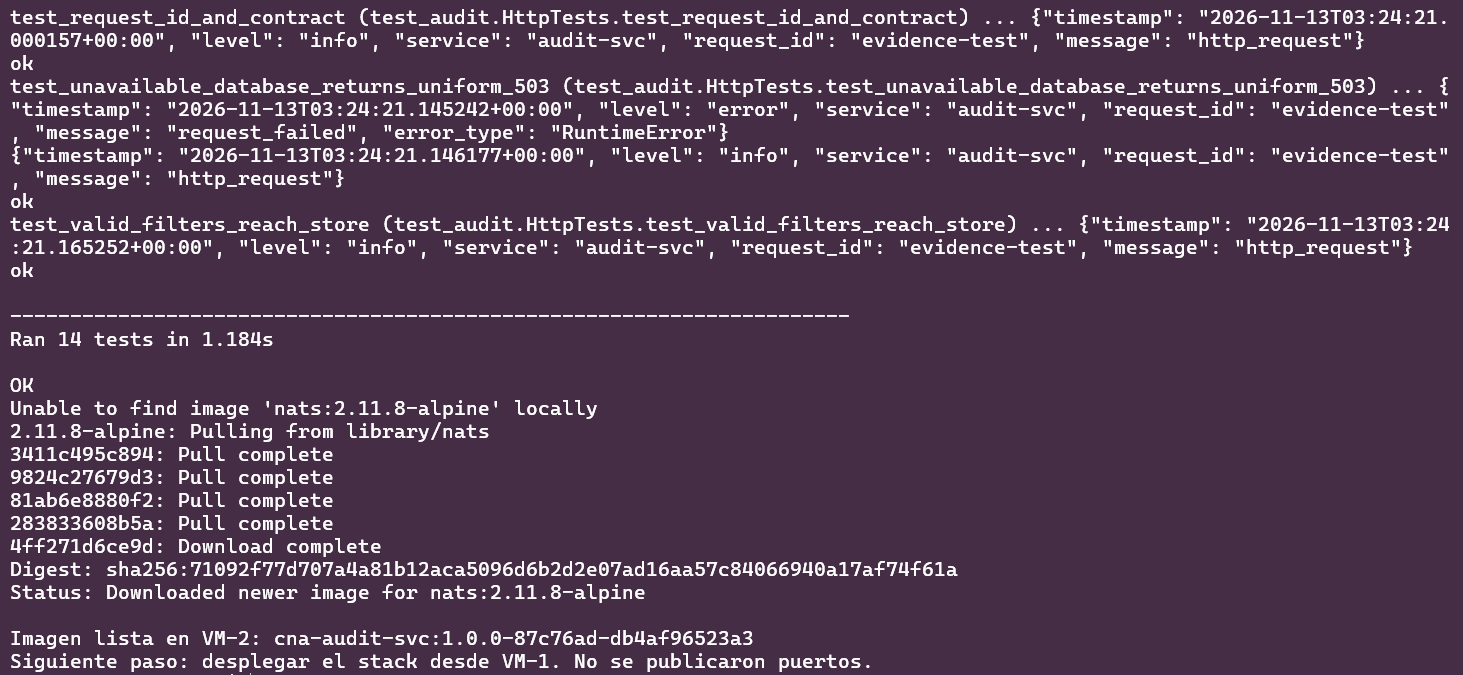
\includegraphics[width=\textwidth,height=5.3cm,keepaspectratio]{../../../cna/docs/evidencias/fase6/preparacion/PRE-B2-VM2-pruebas-Linux.png}
\caption{S2: construcción de la imagen en VM-2 y 14 pruebas automatizadas Linux con resultado OK.}
\label{fig:b2-audit-tests}
\end{figure}

La prueba funcional usa dependencias reales y publica dos mensajes con
el mismo event\_id, sin activar deduplicación de publicación mediante
\texttt{Nats-Msg-Id}. JetStream confirmó las secuencias 1 y 2. Después
de procesar y confirmar ambos mensajes, la consulta devolvió
\texttt{total=1}. El evento es sintético y se identifica como prueba;
no se presenta como una edición real del monolito.

\begin{figure}[H]
\centering
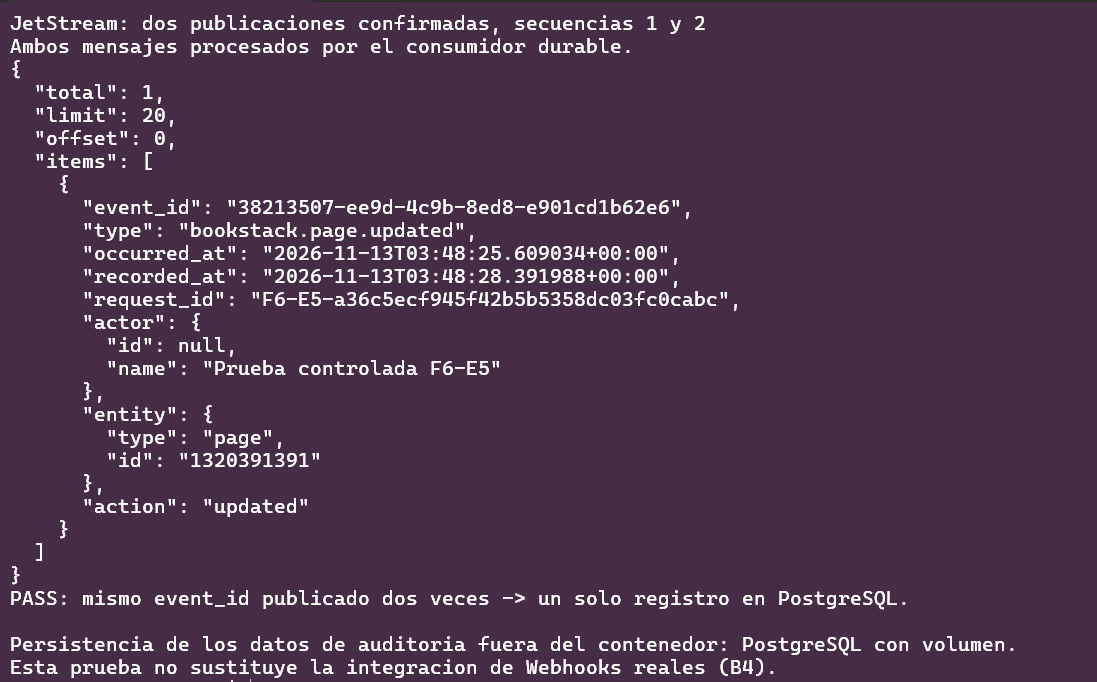
\includegraphics[width=0.90\textwidth,height=6.3cm,keepaspectratio]{../../../cna/docs/evidencias/fase6/preparacion/PRE-B2-VM2-evento-duplicado.png}
\caption{F6-E5 / P37: dos entregas del mismo evento producen un registro en PostgreSQL. El nombre del archivo conserva el prefijo elegido por el equipo.}
\label{fig:F6-E5}
\end{figure}

\clearpage
\paragraph{Persistencia al recrear la tarea y comprobaciones operativas.}
Desde el manager VM-1 se forzó el reemplazo de la tarea S2 mediante:
\begin{quote}\small\ttfamily
docker service update --force --detach=false cna\_audit
\end{quote}
Swarm
reemplazó la tarea \texttt{ua2izsnx8k8i} por \texttt{0nriqr2z2q25},
ambas ubicadas en VM-2. PostgreSQL y NATS permanecieron disponibles.

\begin{figure}[H]
\centering
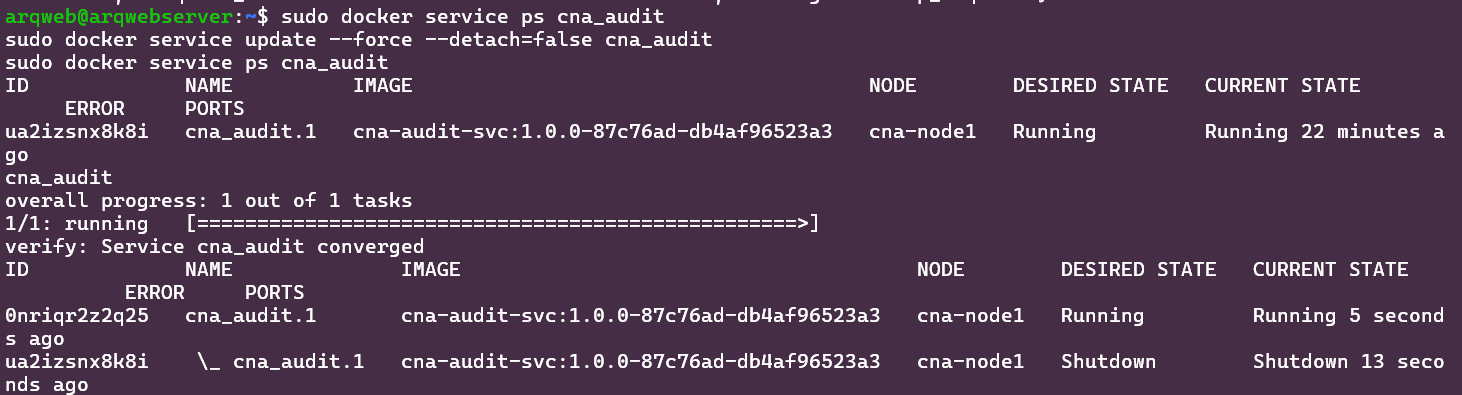
\includegraphics[width=\textwidth,height=4.5cm,keepaspectratio]{../../../cna/docs/evidencias/fase6/preparacion/PRE-B2-VM2-recreacion-tarea.png}
\caption{Reemplazo de S2 solicitado desde VM-1: nueva tarea Running y anterior Shutdown en VM-2.}
\label{fig:b2-audit-recreacion}
\end{figure}

En el nuevo contenedor \texttt{7b140879bca3} se consultó el mismo evento,
sin volver a publicarlo. Se conservó el registro con su fecha original
\texttt{recorded\_at}. Los filtros por entidad/ID y por rango temporal
incluyeron y excluyeron el registro según lo esperado. La herramienta
también validó las series Prometheus y la devolución de X-Request-ID.

\begin{figure}[H]
\centering
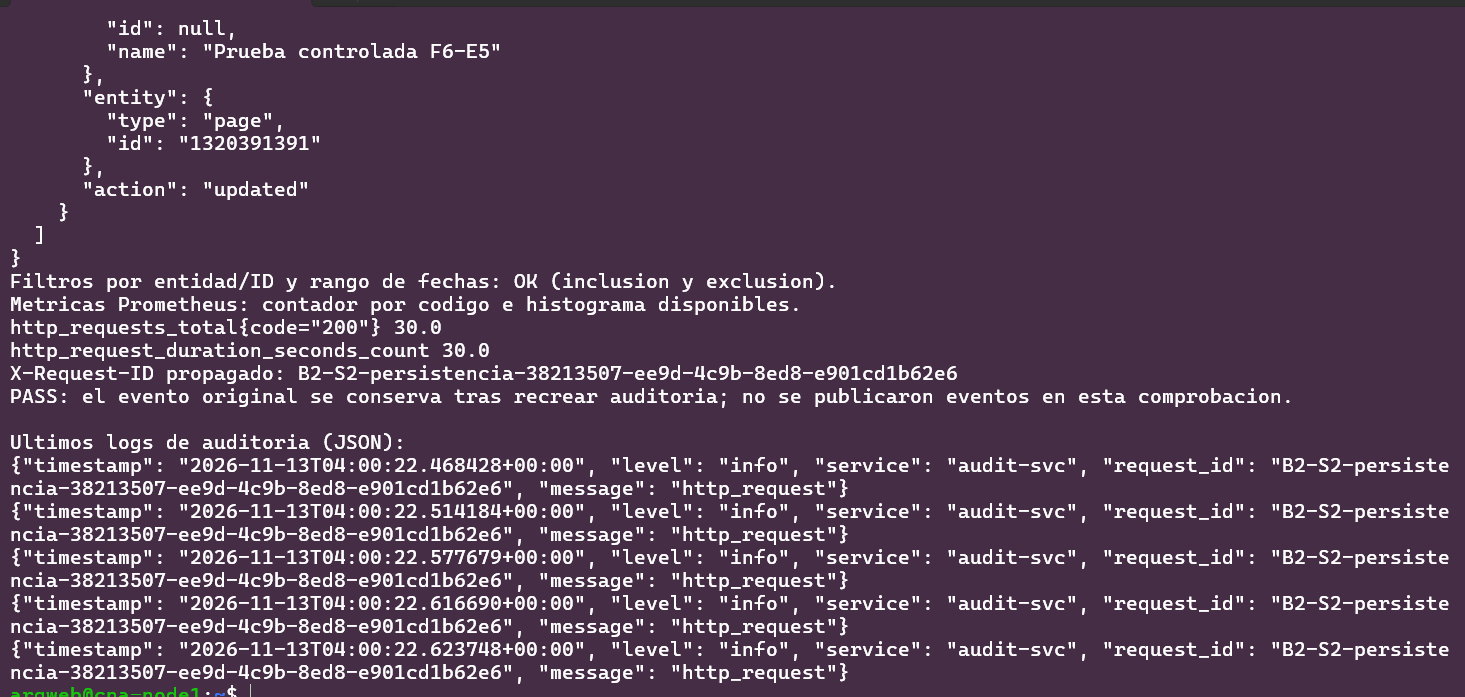
\includegraphics[width=\textwidth,height=6.5cm,keepaspectratio]{../../../cna/docs/evidencias/fase6/preparacion/PRE-B2-VM2-persistencia.png}
\caption{S2: persistencia del evento original, filtros, métricas y logs JSON correlacionados después del reemplazo.}
\label{fig:b2-audit-persistencia}
\end{figure}

\textbf{Resultado de S2:} idempotencia y persistencia satisfactorias, con
sondas, filtros, métricas y correlación comprobados. Las salidas se
conservan junto a las capturas. Permanecen pendientes los Webhooks reales
y la prueba de DLQ (B4). Los avances de búsqueda e integración por gateway
se documentan a continuación; B2 y B5 no se declaran completos.

\clearpage
\subsection{B2.1: búsqueda y actualización por evento real}
\label{sec:b2-search-real}

El servicio S1 se ejecuta en VM-2 y mantiene su índice en PostgreSQL,
separado de MariaDB. Obtiene el contenido por la API REST de BookStack.
La imagen corregida \texttt{cna-search-svc:1.0.0-87c76ad-021cea696896}
superó 35 pruebas Linux, que incluyen las pruebas compartidas y dos
regresiones sobre la espera del consumidor sin mensajes.

\paragraph{F6-E4 / P36: edición y consulta por gateway.}
Con ambas VM activas, se editó desde BookStack la página 3 del libro 2,
reemplazando \texttt{alfa} por \texttt{beta}. El Webhook llegó al puente,
que publicó \texttt{bookstack.page.updated} en JetStream. S1 confirmó
el procesamiento de ese evento en su base. La consulta autenticada por
\texttt{api.bookstack.local}, por la ruta \texttt{/v2/search}, encontró la página con
\texttt{beta} y dejó de encontrarla con \texttt{alfa}.

\begin{figure}[H]
\centering
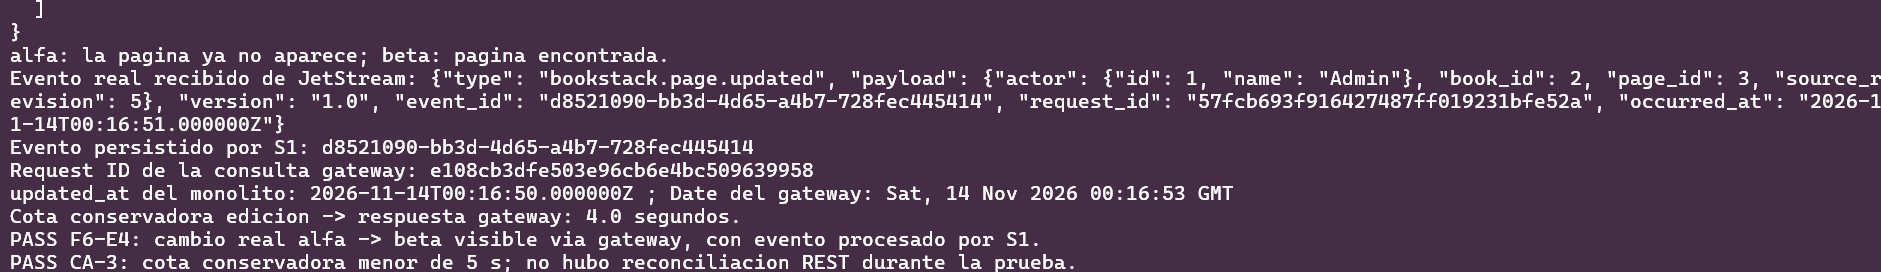
\includegraphics[width=\textwidth]{../../../cna/docs/evidencias/fase6/preparacion/F6-E4-busqueda-edicion-real.png}
\caption{F6-E4 / P36: extracto del resultado de la edición real, evento persistido por S1 y consulta por gateway. La salida textual completa los identificadores.}
\label{fig:F6-E4}
\end{figure}

\paragraph{CA-3: actualización en menos de cinco segundos.}
La fecha de modificación del monolito fue
\texttt{2026-11-14T00:16:50Z}; la cabecera Date de la respuesta del gateway
fue \texttt{00:16:53 GMT}. Al agregar un segundo por la resolución de Date,
la herramienta obtuvo una cota conservadora de \textbf{4,0 segundos},
inferior a cinco. Esta cota corresponde a este ensayo, no a un promedio
ni a un percentil de rendimiento.

Durante la medición se utilizó temporalmente un intervalo de reconciliación
de 3600 segundos y se comprobó que su marca en la base no cambió.
Así se evitó atribuir a eventos una actualización producida por una
reconstrucción REST. Se verificó además que el evento de JetStream era
nuevo y que su identificador estaba registrado por S1.

\paragraph{Trazabilidad y alcance.}
La revisión de origen fue 5. El identificador del evento se conserva completo:
\begin{quote}\small\ttfamily
d8521090-bb3d-4d65-a4b7-728fec445414
\end{quote}
Los campos temporales anteriores se expresan en UTC.
La salida textual se conserva en la carpeta de evidencias de Fase 6,
subcarpeta \texttt{preparacion}, con el nombre:
\begin{quote}\small\ttfamily
F6-E4-busqueda-edicion-real.txt
\end{quote}
F6-E4 y CA-3 resultaron satisfactorios para esta edición. Aún faltan la
comprobación del borrado en S1 y los restantes servicios y criterios de B2;
este resultado tampoco cierra por sí solo B4 ni B5.
